\documentclass[11pt,a4paper]{article}
\usepackage[utf8]{inputenc}
\usepackage[T1]{fontenc}
\usepackage{amsfonts}
\usepackage{amssymb}
\usepackage{mdframed}
\usepackage{tikz}
\usepackage{tkz-tab}
\usepackage{pgfplots}
\usepackage{xcolor}
\usepackage{fancyhdr}
\usepackage{lastpage}
\usepackage[fleqn]{amsmath}
\setlength{\mathindent}{0pt}

% Spécifications du document
\newcommand{\doctitre}{Titre du document} % Ex: Le second degré
\newcommand{\docniveau}{Niveau du doc} % Ex: 1e^{\text{re}}$ Spécialité mathématiques
\newcommand{\doctheme}{Thème du doc } %Ex: Algèbre
\newcommand{\doctype}{Type du doc } % Ex: Démonstrations
\newcommand{\docshorttype}{Type} % Démo

% Couleurs pour les graphiques
\definecolor{dark_green}{HTML}{008000}

% Paramètres du document
\RequirePackage{geometry}
\geometry{tmargin=1cm,bmargin=1.9cm,lmargin=1.9cm,rmargin=1.9cm}
\renewcommand{\familydefault}{\sfdefault}
\setlength{\parindent}{0pt}
\title{\doctitre}
\author{\doctheme - \doctype}
\date{}
\fancypagestyle{custom}{
  \fancyhf{}
  \renewcommand{\headrulewidth}{0pt}
  \lfoot{\doctheme - \docshorttype}
  \cfoot{\doctitre} % Change \titre to \doctitre
  \rfoot{\thepage/\pageref{LastPage}}
}

% Styles pour les mdframed
\mdfdefinestyle{definitionStyle}{
    leftline=true,
    rightline=false,
    topline=false,
    bottomline=false,
    linewidth=2pt,
    linecolor=black,
    innertopmargin=0pt,
    innerbottommargin=0pt,
    innerrightmargin=0pt,
    innerleftmargin=5pt,
}

\mdfdefinestyle{proprieteStyle}{
    linewidth=1pt,
    linecolor=black,
    innertopmargin=5pt,
    innerbottommargin=5pt,
    innerrightmargin=5pt,
    innerleftmargin=5pt,
}

% ----- DEBUT DU DOCUMENT -----
\begin{document}

% Style et numérotation
\maketitle
\pagestyle{custom}
\thispagestyle{custom}

% Sections et sous-sections
\section*{I. Première section}
\subsection*{1. Première sous-section}
\subsection*{2. Deuxième sous-section}
\section*{II. Deuxième section section}
\subsection*{1. Première sous-section}
\subsection*{2. Deuxième sous-section}

% Définition
\begin{mdframed}[style=definitionStyle]
  \textbf{Définition :} ~\\
  % Contenu de la définition
\end{mdframed}

% Propriété
\begin{mdframed}[style=proprieteStyle]
	\textbf{Propriété :} ~\\
  % Contenu de la proriété
\end{mdframed}

% Théorème
\begin{mdframed}[style=proprieteStyle]
	\textbf{Théorème :} ~\\
  % Contenu du Théorème
\end{mdframed}

% Exemple
\textbf{Exemple :} ~\\
% Contenu de l'exemple

% Remarque
\textbf{Remarque :} % Contenu de la remarque

% Tableau de variation
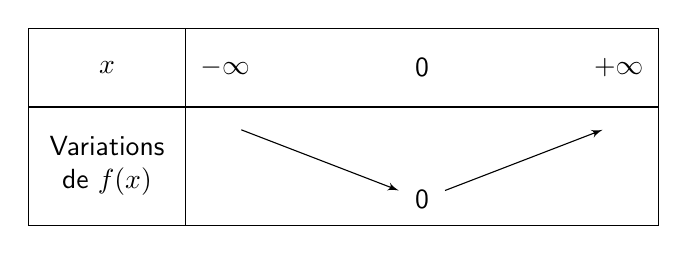
\begin{tikzpicture}[baseline, scale=1, transform shape]
  \tkzTabInit[lgt=2, espcl=2.5]{$x$ / 1 , Variations de $f(x)$ / 1.5}{$-\infty$, 0, $+\infty$}
  \tkzTabVar{+/ , -/ 0, +/ }
\end{tikzpicture}

% Tableau de signe
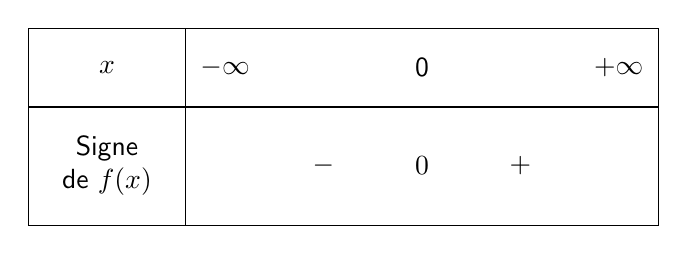
\begin{tikzpicture}[baseline, scale=1, transform shape]
\tkzTabInit[lgt=2, espcl=2.5]{$x$ / 1 , Signe de $f(x)$ / 1.5}{$-\infty$, 0, $+\infty$}
\tkzTabLine{, -, 0, +, }
\end{tikzpicture}

% Tableau de signe et de variation
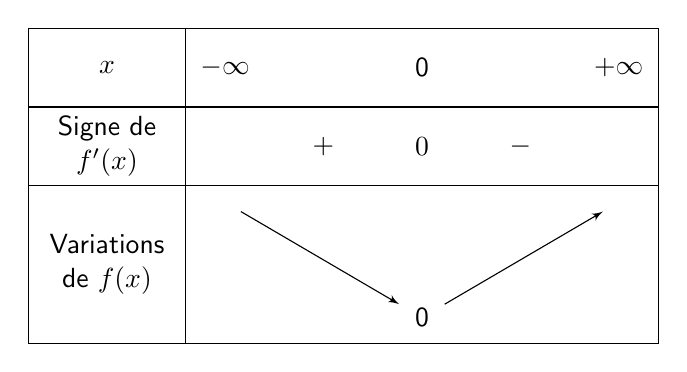
\begin{tikzpicture}
  \tkzTabInit[lgt=2, espcl=2.5]{$x$ / 1 , Signe de $f'(x)$ / 1, Variations de $f(x)$ / 2}{$-\infty$, 0, $+\infty$}
  \tkzTabLine{,+,0,-,} % Signes
  \tkzTabVar{+/ , -/ 0, +/ } % Variations
\end{tikzpicture}

% Graphique
\begin{tikzpicture}
  \begin{axis}[
      axis lines=middle,
      xmin=-2, xmax=2,
      ymin=-2, ymax=4,
      xlabel=$x$,
      ylabel=$y$,
      xtick=\empty,
      ytick=\empty,
    ]
    % Courbe représentative de f(x)=2x²
    \addplot[smooth, thick, red, domain=-2:2]{2*x^2};
    
    % Segments pointillés
    \draw[dashed, thin, blue] (axis cs:0, 2) -- (axis cs:1,2);
    \draw[dashed, thin, dark_green] (axis cs:1, 0) -- (axis cs:1,2);
    
    % Double flèche
    \draw [<->, dark_green, thick] (axis cs: -0.6, 0.4) -- (axis cs: -1.4, 3.4);

    % Noms des points
    \node[label={-90:$\color{dark_green}a$}] at (axis cs:1, 0) {};
    \node[label={180:$\color{blue}f(a)$}] at (axis cs:0, 2) {};
  \end{axis}
\end{tikzpicture}

\end{document}